\documentclass[notheorems,serif,table,compress]{beamer}  %dvipdfm选项是关键,否则编译统统通不过
%%------------------------常用宏包------------------------
%%注意, beamer 会默认使用下列宏包: amsthm, graphicx, hyperref, color, xcolor, 等等
\usepackage{fontspec,xunicode,xltxtra}  % for XeTeX
\usepackage{verbatim}
%\usepackage{mathabx}
\usepackage{latexsym}
\usepackage{amsfonts,amssymb}
\usepackage{styles/iplouclistings}
\usepackage{fancybox}
\usepackage{colortbl}
\usepackage{tcolorbox}
%\usepackage[T1]{fontenc}
%\usepackage{bookman}
\usepackage{subfigure}
\usepackage{hyperref}
\usepackage{listings}
\usepackage{animate}
\usepackage[absolute,overlay]{textpos}
\usepackage{graphicx}
\usepackage{tikz}
\usepackage[americaninductors,europeanresistors]{circuitikz}
\usepackage{tikz}
\usepackage{fancybox}     %% 定义zhushadow时用到
\usepackage{pifont} %ding用到
\newsavebox{\mysaveboxOne}  %%为了在only中使用lstlisting
\newsavebox{\mysaveboxTwo}
\newsavebox{\mysaveboxThree}
\newsavebox{\mysaveboxFour}
\newsavebox{\mysaveboxFive}
\newsavebox{\mysaveboxSix}
\newsavebox{\mysaveboxSeven}
\newcommand\zhushadow[2][purple]{\hskip5pt\shadowbox{\color{#1}\small\kai #2\vspace{3mm}}}

%%------------------------ThemeColorFont------------------------
%% Presentation Themes
% \usetheme[<options>]{<name list>}
%\usetheme{Madrid}
\usetheme{Berkeley}
%% Inner Themes双精度计算
% \useinnertheme[<options>]{<name>}
%% Outer Themes
% \useoutertheme[<options>]{<name>}
%\useoutertheme{miniframes} 
%% Color Themes 
%\usecolortheme[<options>]{<name list>}
%% Font Themes
\usefonttheme{serif}
\setbeamertemplate{background canvas}[vertical shading][bottom=white,top=structure.fg!7] %%背景色, 上25%的蓝, 过渡到下白.
\setbeamertemplate{theorems}[numbered]
\setbeamertemplate{navigation symbols}{}   %% 去掉页面下方默认的导航条.
\usepackage{styles/zhfontcfg}
%\setsansfont[Mapping=tex-text]{文泉驿正黑}  %% 需要fontspec宏包
     %如果装了Adobe Acrobat,可在font.conf中配置Adobe字体的路径以使用其中文字体
     %也可直接使用系统中的中文字体如SimSun,SimHei,微软雅黑 等
     %原来beamer用的字体是sans family;注意Mapping的大小写,不能写错
     %设置字体时也可以直接用字体名,以下三种方式等同:
     %\setromanfont[BoldFont={黑体}]{宋体}
     %\setromanfont[BoldFont={SimHei}]{SimSun}
     %\setromanfont[BoldFont={"[simhei.ttf]"}]{"[simsun.ttc]"}
%%------------------------MISC------------------------
\graphicspath{{figures/}}         %% 图片路径. 本文的图片都放在这个文件夹里了.
%%------------------------listing------------------------
%\lstset{language=[LaTeX]TeX,Python}
%%------------------------正文------------------------
\begin{document}
\XeTeXlinebreaklocale "zh"         % 表示用中文的断行
\XeTeXlinebreakskip = 0pt plus 1pt % 多一点调整的空间
%%----------------------------------------------------------
%% This is only inserted into the PDF information catalog. Can be left
%% out.
%%%
%% Delete this, if you do not want the table of contents to pop up at
%% the beginning of each subsection:
%\AtBeginSection[]{                              % 在每个Section前都会加入的Frame
%  \frame<handout:0>{
%    \frametitle{Contents}\small
%    \tableofcontents[current,currentsubsection]
%  }
%}
%
%\AtBeginSubsection[]                            % 在每个子段落之前
%{
%  \frame<handout:0>                             % handout:0 表示只在手稿中出现
%  {
%    \frametitle{Contents}\small
%    \tableofcontents[current,currentsubsection] % 显示在目录中加亮的当前章节
%  }
%}

\setbeamertemplate{caption}{\raggedright\insertcaption\par}

%%----------------------------------------------------------
\logo{
\includegraphics[scale=0.13]{ouclogo.png}}
\title{Spatial And Intensity Resolution}
%\subtitle{Bottom-Up Saliency Detection Model Based on Human Visual Sensitivity and Amplitude Spectrum}
\subtitle{\color{red}空间分辨率和灰度分辨率}
\author[]{\color{red}{TanLin}}
%\institute[CVBIOUC]
%{
%\small\textcolor{violet}{CVBIOUC\\
%Ocean University of China\\
%\url{http://vision.ouc.edu.cn/~zhenghaiyong}}
%}
\date[]{\color{red}August 15,2016}
%\titlegraphic{
%\includegraphics[height=1.0cm]{ouc-logo.jpg}}
\frame{ \titlepage }
%%----------------------------------------------------------
%\section*{Contents}
\frame{\frametitle{Contents}\tableofcontents}
%%----------------------------------------------------------
\def\hilite<#1>{\temporal<#1>{\color{blue!15}}{\color{black}}{\color{black}}}
\newcommand{\shadow}[2][purple]{\hskip5pt\shadowbox{\color{#1}\small \kai #2\vspace{3mm}}}
\newcommand{\colorrbox}[2][purple]{\doublebox{\color{#1}\small \kai#2}}

%============================================================================

\section{Resolution}

%==========================================================================


%\begin{frame}[fragile]
%\frametitle{What?}
 %   \begin{figure}
 %   \includegraphics[width=0.8\linewidth]{edgeseg.png} 
  %  \end{figure}
%\end{frame}


\subsection{Classification Of Resolution }

\begin{frame}
\frametitle{Classification Of Resolution }
    %\begin{tcolorbox}[colback=red!5,colframe=blue!75!black]
        %\begin{figure}
         %   \begin{minipage}[t]{0.3\linewidth}
          %  \centering
          %  \caption{original image}
           % \includegraphics[width=1\linewidth]{src.png} 
            %\end{minipage}
            %\begin{minipage}[t]{0.3\linewidth}
            %\centering
            %\caption{edge}
            %\includegraphics[width=1\linewidth]{edge.png} 
            %\end{minipage}
            %\begin{minipage}[t]{0.3\linewidth}
            %\centering
            %\caption{boundary}
            %\includegraphics[width=1\linewidth]{bounary.png} 
            %\end{minipage}
        %\end{figure}
    %\end{tcolorbox}
\begin{itemize}
  \item 分辨率是度量位图图像内数据量多少的一个参数,例如显示屏的分辨率1024×768(15英寸);输出图形的大小7×6英寸。
  \item 分辨率分为显示分辨率和图像分辨率
   
   \item 显示分辨率(屏幕分辨率):值得是显示器能显示像素的多少,屏幕图像的清晰度。像素越多,图像越清晰。

   \item 图像分辨率:Image resolution is the detail an image holds.其指图像中存储的信息量,它还与文件的大小成正比。
  
  ~~简而言之,单位英寸所包含的像素点数,主要以ppi衡量。

  {\color{blue}Image resolution 种类很多,这里主要研究Spatial resolution和Intensity resolution对图像的影响效果。}

  \end{itemize}.
\end{frame}
 
 
\subsection{Resolution Unit}

\begin{frame}
\frametitle{Resolution Unit}
Resolution的表示单位:dpi,ppi。
    \begin{itemize}
        \item {\color{blue}{\textbf{dpi:}}}英文全称是dots per inch。在图像处理主要指的是打印机的输出分辨率,取样可显示或输出点的数目。分为垂直分辨率和水平分辨率。
        \item {\color{blue}{\textbf{ppi:}}}英文全称是pixels per inch。一张照片或者图像输入的分辨率。
       \item pixels是构成图像的单元,它是有无数的sub—pixels构成,这与dots不等价的。屏幕上每英寸像素(ppi)的数量是固定的数量。显示屏分辨率已经知道了,打印的时候,你改变ppi,只会改变尺寸,但像素大小不变。所以改变图像的分辨率是改变单位面积内的像素点数(dpi),而不是改变ppi。
    \end{itemize}
    %\begin{figure}
     %   \begin{minipage}[t]{0.4\linewidth}
     %   \centering
      %  \includegraphics[width=1\linewidth]{0_0_284.jpg} 
       % \end{minipage}
        %\begin{minipage}[t]{0.4\linewidth}
        %\centering
        %\includegraphics[width=1\linewidth]{noise.png} 
        %\end{minipage}
    %\end{figure}
\end{frame}

\section {Spatial Resolution}
\subsection{Spatial Resolution Introduction}

\begin{frame}
\frametitle{Spatial Resolution}
 
    \begin{itemize}
        \item {\color{blue}Spatial Resolution:} the smallest discernble detail in an image.定义是独立的单位长度的像素值数目。
        
   在研究空间分辨率时,在不同研究领域时,它指的不同。对于数字图像,指的是用于图像在构造中的像素数目,定义是独立的单位长度的像素值数目。即:
 
     \item  像素的数目决定空间的分辨率,空间分辨率决定图像的清晰度。

    \end{itemize}
\end{frame}
\subsection{Research Ideas}
\begin{frame}
\frametitle{Research Ideas}
    \begin{itemize}
        \item 这次主要是研究的是降低空间分辨率对于图像细节的影响。降低图像分辨率主要通过缩小图像的尺寸。因为缩小之后,在放大原先尺寸,单位面积内的像素点就减少了,从而图像的空间分辨率也降低了。
        \item {\color{blue}将彩色图像读入,访问出RGB三个通道的像素值矩阵,一开始以4*4的正方形为单位对矩阵求均值,然后将求出的均值存放在另一个与类型相同,但是尺寸为原图像的四分之一的矩阵之中,像素也就减少为原来的四分之一。设原图像的分辨率为1250dpi,那么此时分辨率为300dpi。同样的道理分别以8*8,16*16的正方形为单位对矩阵求均值,将均值放在尺寸为原来的八分之一、十六分一的矩阵中,此时的分辨率为150dpi和72dpi。}

 ps:图像处理中一般都是以二的倍数进行缩减的。
    \end{itemize}
   
\end{frame}


\subsection{Code}

\begin{frame}
\frametitle{Code}
\href{code/resolution.cpp}{\color{red}具体的代码如下:}
  
\end{frame}
\subsection{Running Results}
\begin{frame}
\frametitle{Running Results}
\begin{figure}
        \begin{minipage}[t]{0.4\linewidth}
        \centering
        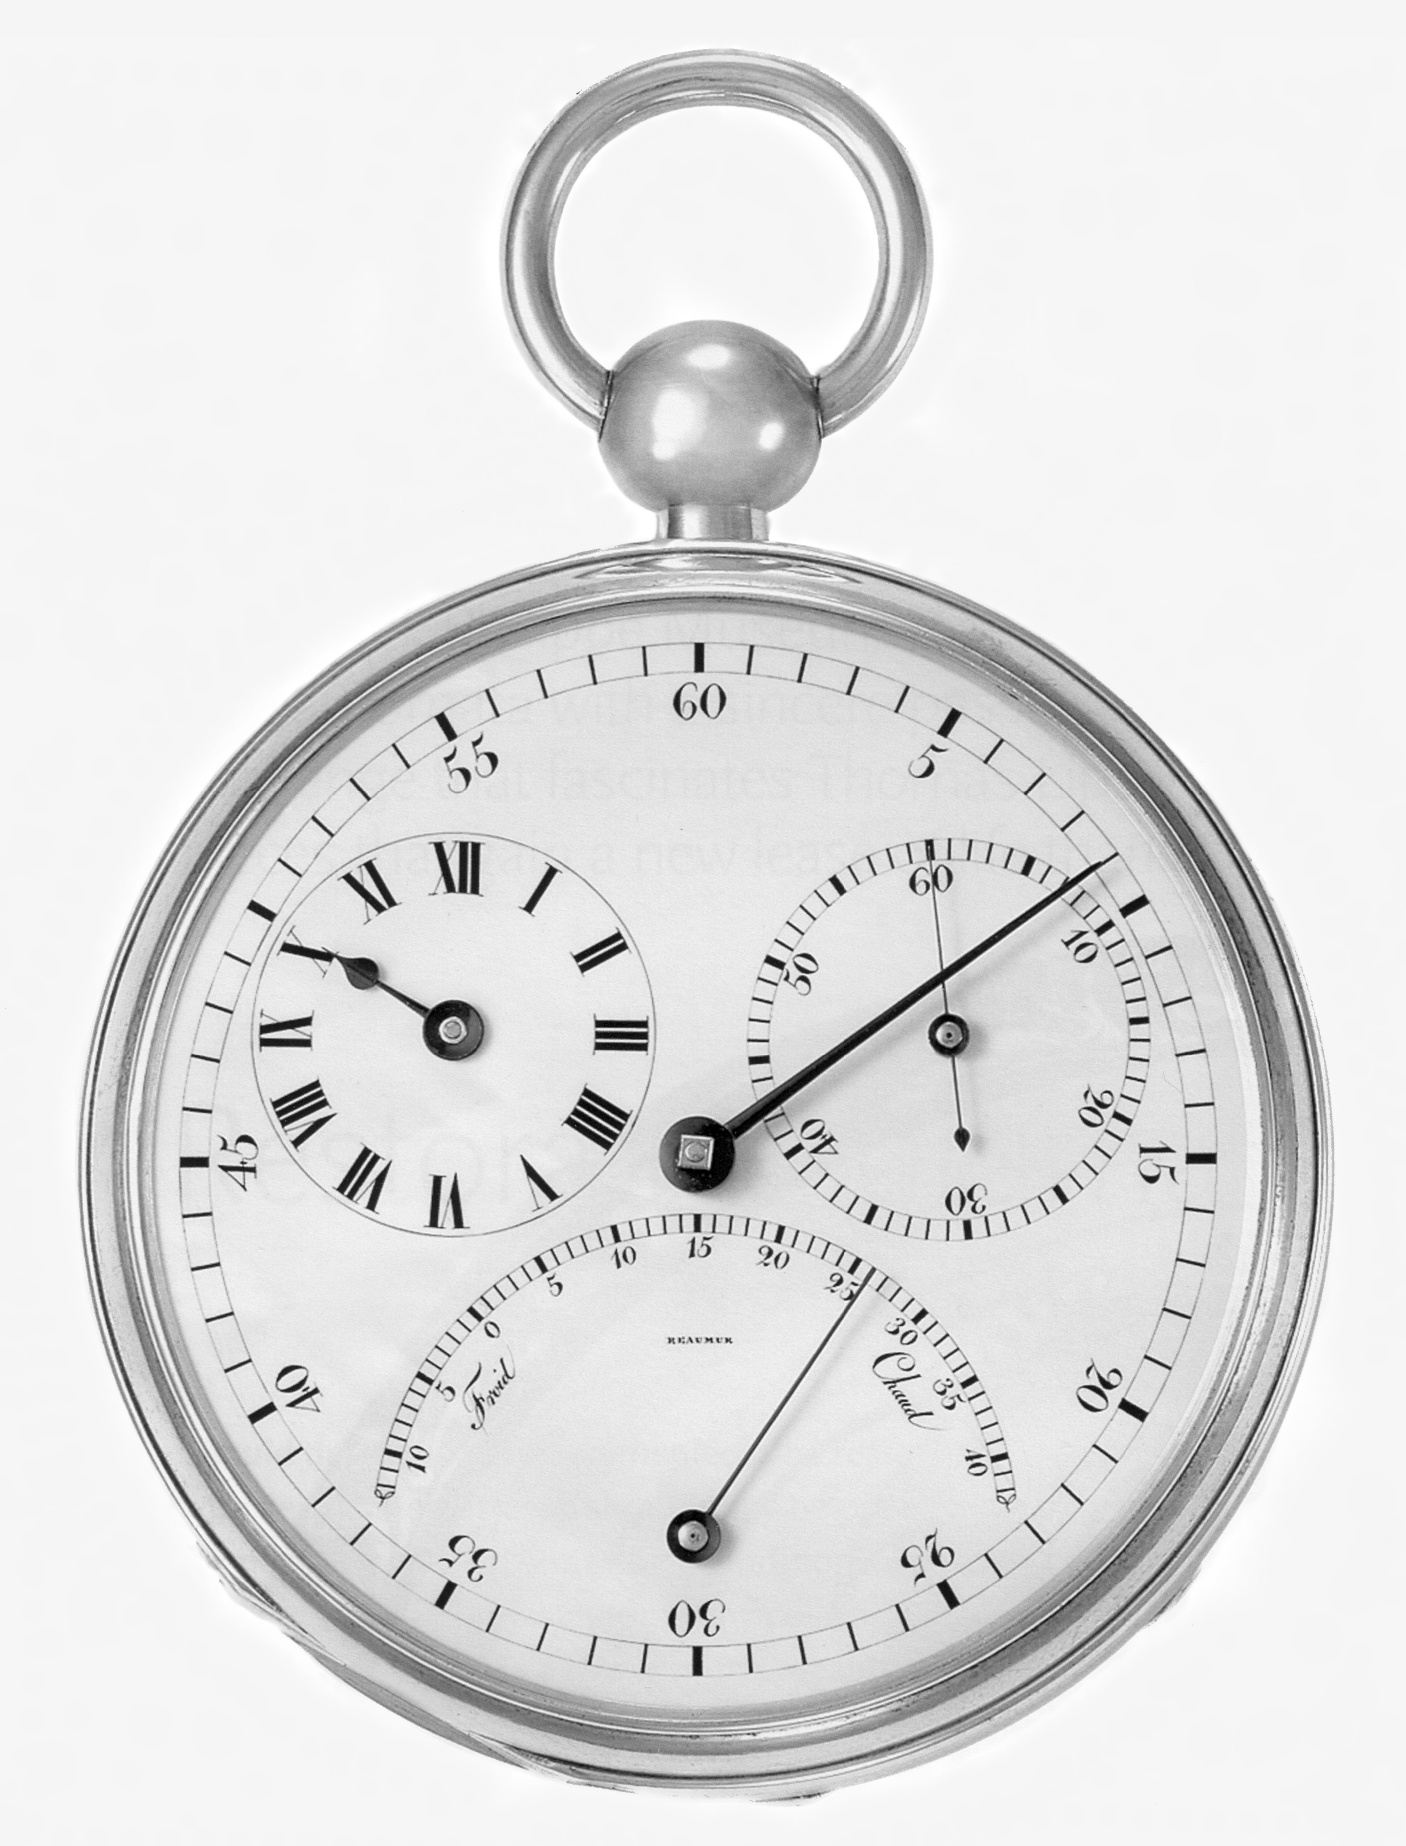
\includegraphics[width=0.7\linewidth]{1250dpi.jpg} 
        \end{minipage}
        \begin{minipage}[t]{0.4\linewidth}
        \centering
        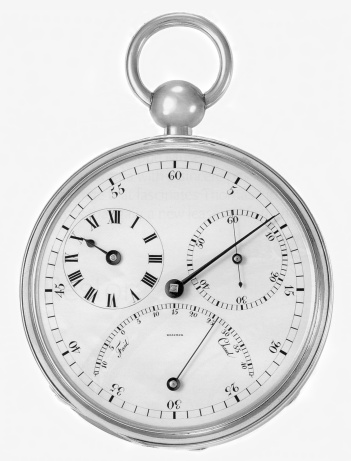
\includegraphics[width=0.7\linewidth]{300dpi.jpg} 
        \end{minipage}
        \begin{minipage}[t]{0.4\linewidth}
        \centering
        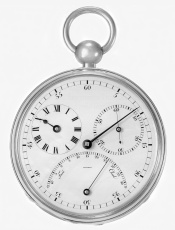
\includegraphics[width=0.7\linewidth]{150dpi.jpg} 
        \end{minipage}
        \begin{minipage}[t]{0.4\linewidth}
        \centering
        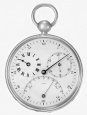
\includegraphics[width=0.7\linewidth]{72dpi.jpg} 
        \end{minipage}
    \end{figure}
\end{frame}
\begin{frame}
\frametitle{Running Results}
  从上面图可以看出来,第一幅图1406*1846,依次尺寸变为四分之一、八分之一、十六分之一,将四幅图以同比例展示可以发现,尺寸越小,图像越模糊,第四幅图已经失真。因为尺寸扩大后,单位面积里的像素点少了,细节也小了,所以空间分辨率也降低了,图像变得模糊。
\end{frame}

%============================================================================
\section{Intensity Resolution}

%===============================================================================
\subsection{Intensity Resolution Introduction}
\begin{frame}
\frametitle{Intensity Resolution Introduction}
\begin{itemize}
\item {\color{blue}Intensity Resolution:}the smallest discernible change in intensity level.定义是在一个图像上阴影或者灰度级上可预见的或确定性的,用于量化灰度的比特数。
\item 简而言之,改变图像的灰度分辨率就是改变灰度级的比特数k。

\end {itemize}
\end{frame}

\subsection{Research Ideas}
\begin{frame}
\frametitle{Research Ideas}
    \begin{itemize}
\item {\color{blue}假设灰度级是256,比特数k=8,要想k=7,就是将颜色的256个等级像素值进行减半。我们可以这要这样理解:

 像素是0--1的像素值为0;\\
 像素是2--3的像素值为2;\\
 像素是4--5的像素值为4;\\
 像素是6--7的像素值为6;\\
......\\
 像素是252--253的像素值为252;\\
 像素是254--255的像素值为254;\\}
\item {\color{blue}具体操作是:}{\color{red}(data/2)*2}{\color{blue},这样有256级像素值就变成了128级,k=7,颜色由原来的256*256*256变成128*128*128。同样道理,k=6...k=1就可以求出来了。}
\end{itemize}
\end{frame}
\subsection{Code}

\begin{frame}
\frametitle{Code}
\href{code/intensity.cpp}{\color{red}具体的代码如下:}
\end {frame}
\subsection{Running Results}
\begin{frame}
\frametitle{Running Results}
\begin{figure}
        \begin{minipage}[t]{0.4\linewidth}
        \centering
        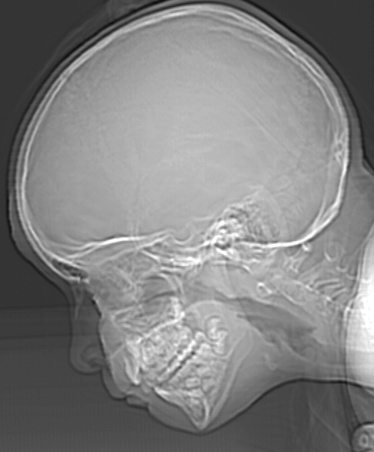
\includegraphics[width=0.8\linewidth]{k=8.jpg} 
        \end{minipage}
        \begin{minipage}[t]{0.4\linewidth}
        \centering
        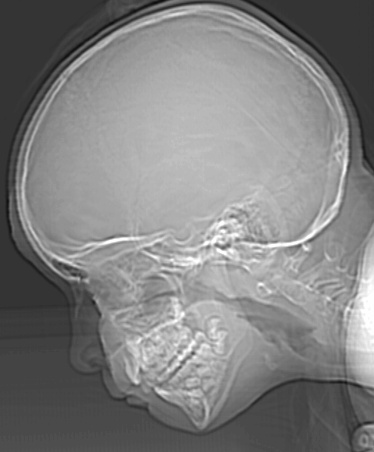
\includegraphics[width=0.8\linewidth]{k=7.jpg} 
        \end{minipage}
        \begin{minipage}[t]{0.4\linewidth}
        \centering
        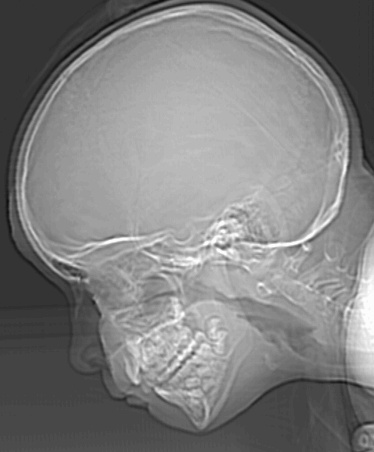
\includegraphics[width=0.8\linewidth]{k=6.jpg} 
        \end{minipage}
        \begin{minipage}[t]{0.4\linewidth}
        \centering
        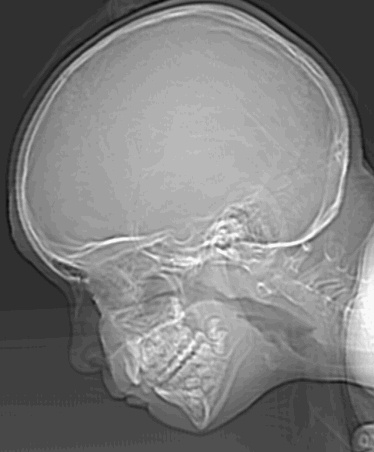
\includegraphics[width=0.8\linewidth]{k=5.jpg} 
        \end{minipage}
       
\end{figure}
\end{frame}
\begin{frame}
\frametitle{Running Results}
\begin{figure}
        \begin{minipage}[t]{0.4\linewidth}
        \centering
        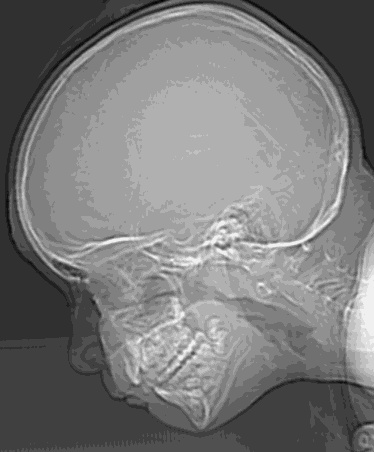
\includegraphics[width=0.8\linewidth]{k=4.jpg} 
        \end{minipage}
        \begin{minipage}[t]{0.4\linewidth}
        \centering
        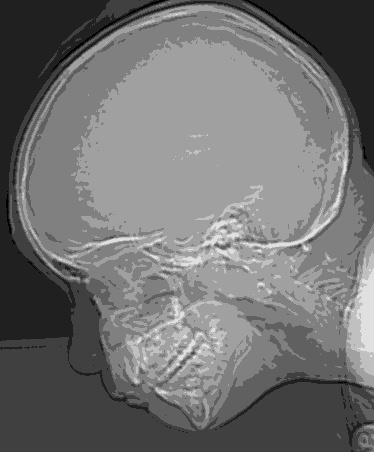
\includegraphics[width=0.8\linewidth]{k=3.jpg} 
        \end{minipage}
        \begin{minipage}[t]{0.4\linewidth}
        \centering
        
\includegraphics[width=0.8\linewidth]{k=2.jpg} 
        \end{minipage}
        \begin{minipage}[t]{0.4\linewidth}
        \centering
        
\includegraphics[width=0.8\linewidth]{k=1.jpg} 
        \end{minipage}
       

    \end{figure}
\end{frame}
\begin{frame}
\frametitle{Running Results}
  从上面图可以看出来,在保证图像的像素大小不变,前三副没啥差别。在第四副也就是k=5灰度级为32时,在头盖骨内有一组类似细小山脊状结构,随着k的减少越来越明显。当k=1灰度级为二时,图像只有两种颜色就是白色黑色,也就是一副二值图像。
\end{frame}
\end{document}
